\chapter{Architecture de MetaDONE}
\label{chap:architecture}

L'architecture de l'outil MetaDONE repose sur une structure en trois couches : la couche présentation (\texttt{metadone\_bundle\_client}), la couche logique métier (\texttt{metadone\_bundle\_metabusiness}) et la couche repository (\texttt{metadone\_bundle\_repository}). Afin de garantir une grande modularité et extensibilité, MetaDONE s'appuie sur Eclipse Equinox, une implémentation du standard OSGi. Ce framework permet de découper l'application en composants dynamiques et indépendants appelés bundles. L'un des atouts majeurs de cette architecture est la possibilité d'installer, de démarrer, de mettre à jour ou d'arrêter ces modules au moment de l'exécution, sans nécessiter d'interruption de service.

Dans les sous-sections suivantes, nous développerons les langages de modélisation de MetaDONE, MetaL$_1$ et MetaL$_2$, le pattern \emph{Design by Contract} utilisé dans toute l'application, ainsi chacun des bundles présentés à la figure~\ref{fig:bundles-overview}.

\paragraph{Note sur l'usage d'outils d'assistance.}
Les figures représentant les bundles MetaDONE (figures~\ref{fig:bundles-overview}, \ref{bundle-client}, \ref{bundle-MB}, \ref{bundle-repo} et~\ref{bundle-common}) ainsi que le diagramme du langage MetaL$_2$ (figure~\ref{fig:metaL2}) ont été générées à partir de spécifications PlantUML produites avec l'assistance d'un modèle de langage. Chaque diagramme a été relu et corrigé manuellement pour assurer la fidélité au code source.

\begin{figure}[h]
\centering
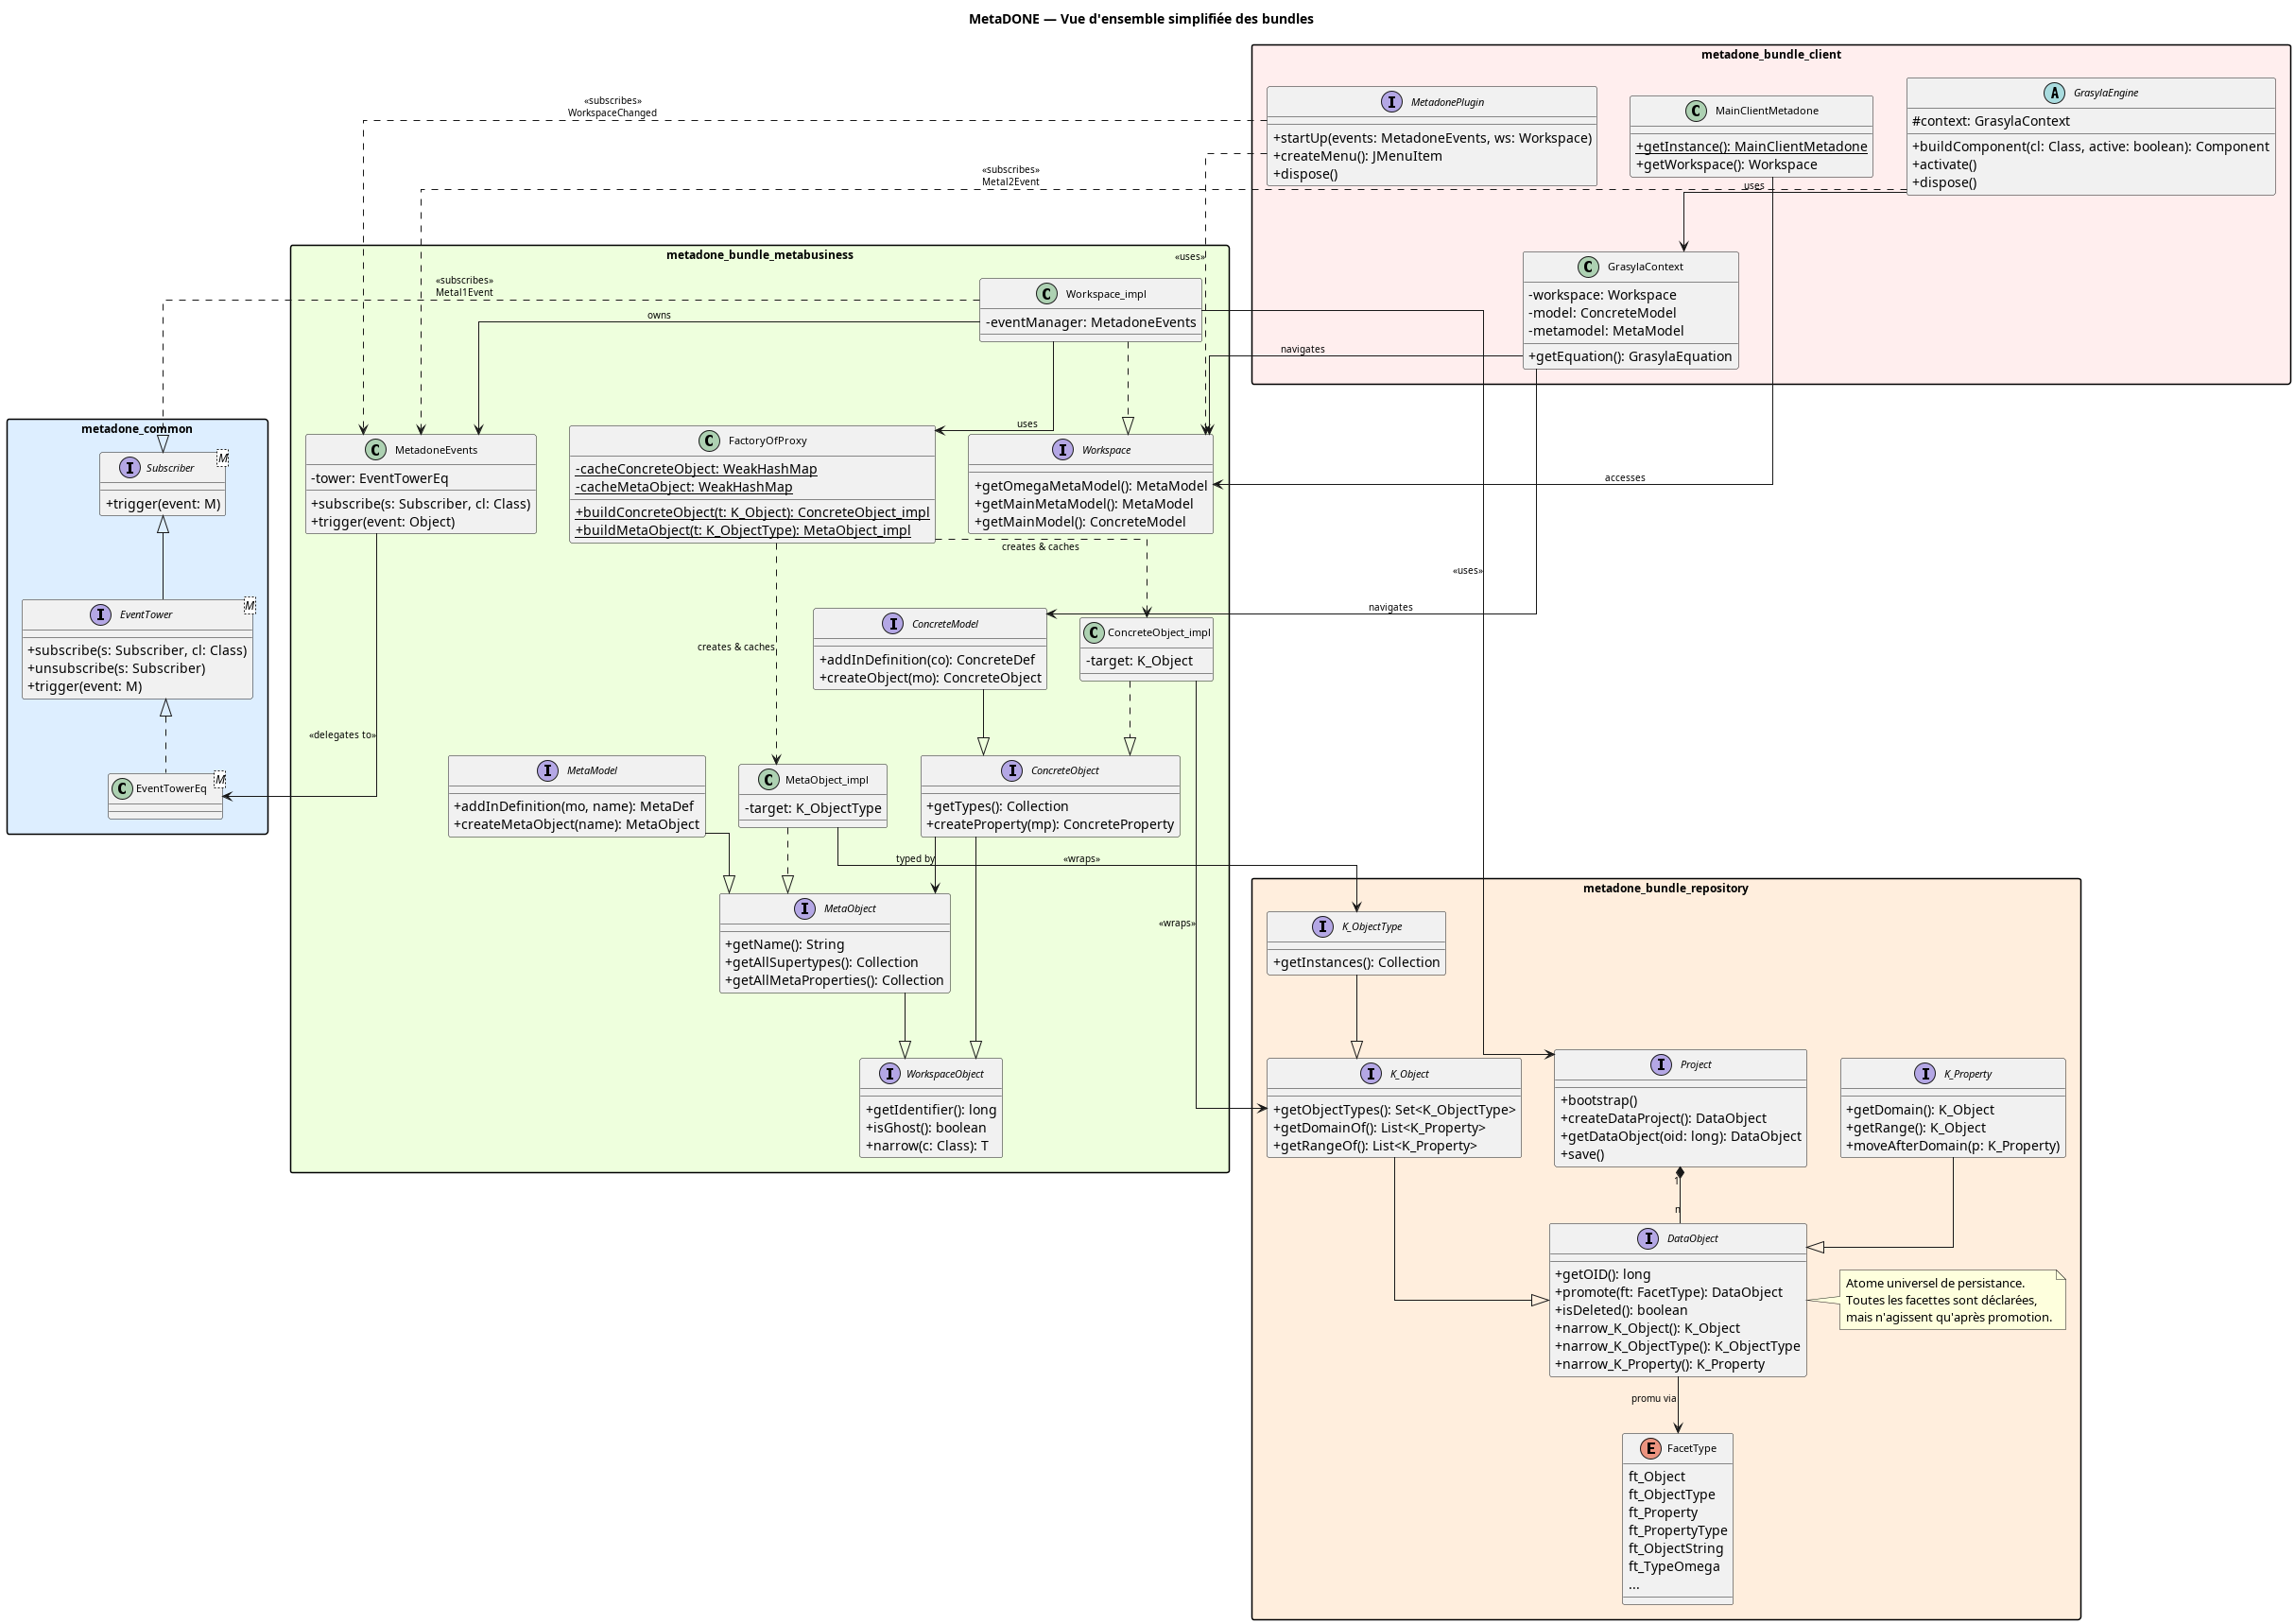
\includegraphics[width=0.8\textwidth]{img/architecture/bundles-overview.png}
\caption{Bundles MetaDONE}
\label{fig:bundles-overview}
\end{figure}

% ---------------------------------------------------------------
% ---------------------------------------------------------------
\section[MetaL$_1$ et MetaL$_2$]{MetaL$_1$ et MetaL$_2$ : les deux niveaux de MetaDONE}
\label{sec:metal1-2}
% ---------------------------------------------------------------
% ---------------------------------------------------------------

MetaDONE repose sur une architecture à deux spécifications complémentaires, inspirée du standard MOF (voir section~\ref{sec:dsl-dsml}). MetaL$_1$ constitue le noyau formel du framework : il définit un ensemble minimal de construits de bas niveau sur lequel tout le reste est bâti. MetaL$_2$ est le langage de modélisation construit entièrement sur ce substrat ; il se décline en deux couches d'instanciation : la couche méta-modèle (niveaux M2 et M3) et la couche concrète (niveau M1). Ces deux spécifications structurent l'ensemble du framework et constituent le vocabulaire central que l'on retrouve à travers tous les bundles.

% ---------------------------------------------------------------
\subsection{MetaL$_1$ : le noyau formel}
\label{sec:metal1}
% ---------------------------------------------------------------


MetaL$_1$ est la spécification formelle du dépôt de MetaDONE. Elle se réduit à un unique construit, le \texttt{DataObject}, et à un ensemble fini de \emph{facettes} (\texttt{K\_Object}, \texttt{K\_ObjectType}, \texttt{K\_Property}, \texttt{K\_PropertyType}, ainsi que les facettes de type primitif) qu'un \texttt{DataObject} peut acquérir cumulativement~\cite{englebert_metal1}. À ce niveau, aucune notion de \og méta-objet \fg{} ni d'\og objet concret \fg{} n'existe encore : ces sémantiques sont l'apanage de MetaL$_2$, qui se construit sur le substrat de MetaL$_1$. Dans MetaDONE, MetaL$_1$ est implémenté par le bundle \texttt{metadone\_bundle\_repository} ; MetaL$_2$ n'en est qu'un client.


\subsection{MetaL$_2$ : la couche méta-modèle (M2/M3)}
\label{sec:metal2}

MetaL$_2$ est la couche de description. Elle permet de définir la structure d'un domaine : quels types d'objets existent, quels attributs ils portent et quelles relations les lient. Les concepts fondamentaux de cette couche sont décrits ci-dessous et sont représentés à la figure~\ref{fig:metaL2}.

Un \texttt{MetaObject} représente un type du domaine modélisé, analogue à une classe dans un langage orienté objet. Il supporte l'héritage multiple via les relations de sous-typage (\texttt{getAllSupertypes()}, \texttt{getAllSubtypes()}) et expose l'ensemble de ses attributs hérités (\texttt{getAllMetaProperties()}).

Un \texttt{MetaModel} est un espace de noms regroupant des \texttt{MetaObject}. Il joue le rôle de \emph{package} ou de \emph{namespace} et fournit les opérations de création des éléments qu'il contient. L'appartenance d'un \texttt{MetaObject} à un \texttt{MetaModel} est matérialisée par une instance de \texttt{MetaDef}, qui enrichit cette relation de trois métadonnées~: un booléen \texttt{canNotBeShared} interdisant le partage de l'objet entre plusieurs modèles ; un booléen \texttt{isDependentOn} précisant si l'objet doit être supprimé en cascade lors de la suppression du modèle ; et un booléen \texttt{isHidden} permettant de masquer les concepts techniques dans l'interface utilisateur. %La spécification formelle~\cite{englebert_metal2} mentionne une quatrième propriété (\texttt{nickname}, pour renommer localement un méta-objet) qui n'a pas été implémentée dans la version actuelle de MetaDONE.

Une \texttt{MetaProperty<T>} est un attribut typé d'un \texttt{MetaObject}. Elle porte la cardinalité, le type de valeur attendu et, le cas échéant, une liste de valeurs énumérées autorisées.

Un \texttt{MetaRole} est une relation binaire dirigée entre deux \texttt{MetaObject} : un domaine et un codomaine (\emph{range}). Il précise la cardinalité de la relation (1-1, 1-N, N-1, N-N) et si les collections aux deux extrémités sont ordonnées. Chaque extrémité porte un nom de navigation (\texttt{getDomainName()}, \texttt{getRangeName()}).

Il convient de souligner que \texttt{MetaProperty}, \texttt{MetaRole} et \texttt{MetaModel} héritent tous de \texttt{MetaObject}: ils sont eux-mêmes des méta-objets, et peuvent à ce titre participer aux mêmes mécanismes de typage et de réflexivité.

\begin{figure}[h]
\centering
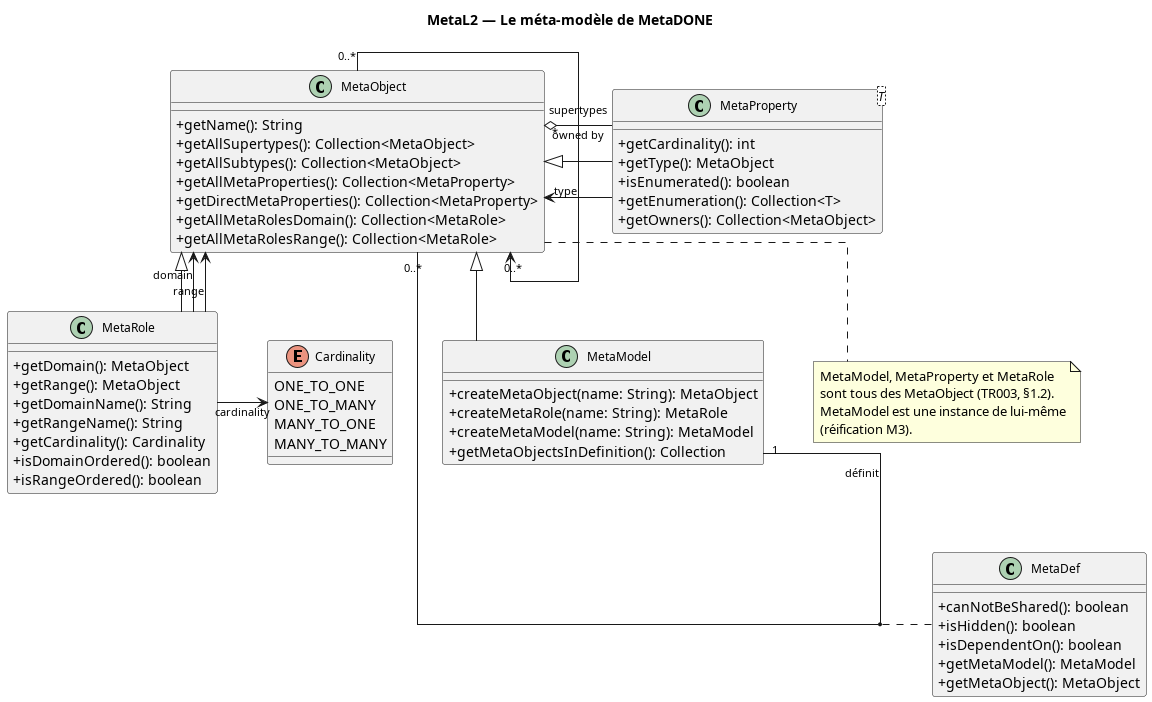
\includegraphics[width=0.9\textwidth]{img/architecture/metal2.png}
\caption{Langage de modélisation MetaL$_2$}
\label{fig:metaL2}
\end{figure}

% ---------------------------------------------------------------
\subsection{MetaL$_2$ : la couche concrète (M1)}
\label{sec:couche-concrete}
% ---------------------------------------------------------------

La couche concrète est la couche d'instanciation de MetaL$_2$. Elle contient les objets effectivement manipulés lors de l'exécution d'un outil construit avec MetaDONE. Chaque concept y est le miroir concret de son homologue de la couche méta-modèle : là où la couche méta-modèle emploie les construits de type de MetaL$_1$ (\texttt{K\_ObjectType}, \texttt{K\_PropertyType}), la couche concrète repose sur les construits d'instance (\texttt{K\_Object}, \texttt{K\_Property}).

Un \texttt{ConcreteObject} est une instance d'un ou plusieurs \texttt{MetaObject}. Il peut posséder plusieurs types simultanément, potentiellement issus de méta-modèles différents (\texttt{getTypes()}, \texttt{getType(MetaModel)}). Un \texttt{ConcreteModel} est un conteneur de \texttt{ConcreteObject}, instance d'un \texttt{MetaModel}. De même qu'un \texttt{MetaDef} lie un \texttt{MetaObject} à son méta-modèle, un \texttt{ConcreteDef} lie un objet concret à son modèle.

Une \texttt{ConcreteProperty<T>} est la valeur effective d'une \texttt{MetaProperty} pour un \texttt{ConcreteObject} donné. Un \texttt{ConcreteRole} est le lien concret entre deux \texttt{ConcreteObject}, instance d'un \texttt{MetaRole}.

% ---------------------------------------------------------------
\subsection{Le \texttt{Workspace} comme point d'entrée}
\label{sec:workspace}
% ---------------------------------------------------------------

Le \texttt{Workspace} est l'interface racine qui donne accès aux deux couches. Il expose systématiquement deux instances de chaque niveau :

\begin{itemize}
    \item \texttt{getOmegaMetaModel()} et \texttt{getOmegaModel()} : le méta-modèle et le modèle prédéfinis par MetaDONE, en lecture seule, qui contiennent les types primitifs (String, Integer, Float, Boolean, Char) ainsi que les méta-types du framework.
    
    \item \texttt{getMainMetaModel()} et \texttt{getMainModel()} : le méta-modèle et le modèle définis par l'utilisateur ou le plugin, dans lesquels sont créés les types du domaine et leurs instances.
\end{itemize}

% ---------------------------------------------------------------
\subsection{Un premier regard sur la réflexivité}
\label{sec:reflexivite-intro}
% ---------------------------------------------------------------

Un trait caractéristique de cette architecture est que \texttt{MetaProperty}, \texttt{MetaRole} et \texttt{MetaModel} héritent tous de \texttt{MetaObject}, et que symétriquement \texttt{ConcreteProperty}, \texttt{ConcreteRole} et \texttt{ConcreteModel} héritent tous de \texttt{ConcreteObject}. Un méta-modèle est donc lui-même un méta-objet, et un modèle concret est lui-même un objet concret : ils peuvent avoir des types, des propriétés et participer à des rôles au même titre que n'importe quel élément de MetaL$_2$.  Cette propriété, dit \emph{réflexive}, permet à MetaDONE de se décrire lui-même avec ses propres outils : le méta-modèle Omega décrit les concepts de MetaL$_2$ (\texttt{MetaObject}, \texttt{MetaRole}, etc.) comme des \texttt{MetaObject} ordinaires. Les implications de cette réflexivité sur l'architecture et les performances seront développées en section~\ref{sec:reflexivite}.

% ---------------------------------------------------------------
\section{Principes de développement}
% ---------------------------------------------------------------

Avant de décrire les bundles, il convient de présenter les principes architecturaux qui structurent de façon uniforme toute l'implémentation de MetaDONE.

% ---------------------------------------------------------------
\subsection{Design by Contract}
\label{sec:dbc}
% ---------------------------------------------------------------

MetaDONE applique systématiquement le patron \emph{Design by Contract} dans l'ensemble de ses couches d'implémentation. Ce
patron repose sur une séparation stricte entre les responsabilités des
méthodes publiques et celles des méthodes privées.

Chaque opération est donc décomposée en deux niveaux :
\begin{enumerate}
    \item \textbf{La méthode publique} constitue la frontière du contrat.
    Elle valide de façon défensive l'ensemble des préconditions de son
    appelant : nullité des arguments, cohérence des états, unicité des
    éléments. En cas de violation, elle lève une \texttt{BadPreCondition} (ou sa spécialisation \texttt{NullArgument}).
    Une fois toutes les préconditions satisfaites, elle délègue le travail effectif à la méthode privée correspondante, conventionnellement préfixée par le caractère \texttt{\_}.

    \item \textbf{La méthode privée} opère sous hypothèse que les
    préconditions ont déjà été vérifiées par son appelant et utilise des \texttt{assert} Java pour documenter et vérifier ses invariants en mode débogage. Ces assertions peuvent être désactivées en production
    sans aucun coût fonctionnel.
\end{enumerate}

\paragraph{Exemple 1 — \texttt{ConcreteObject\_impl.getType()}.}
La méthode publique \texttt{getType} ne fait que vérifier que son
argument n'est pas nul avant de déléguer à \texttt{\_getType} :

\begin{lstlisting}[language=Java]
// Methode publique : verification defensive
public MetaObject getType(MetaModel metamodel) throws BadPreCondition {
    NullArgument.check(metamodel);   // leve BadPreCondition si null
    return _getType(metamodel);      // delegation au prive
}

// Methode privee : assertions internes
private MetaObject _getType(MetaModel metamodel) {
    // metamodel != null garanti par l'appelant public
    final Set<MetaObject> allTypesOfThis = new HashSet<MetaObject>();
    for (final K_ObjectType type : target.getObjectTypes()) { ... }
    assert allTypesOfThis.size() > 0;  // invariant verifie en debug
    ...
}
\end{lstlisting}

\paragraph{Exemple 2 — \texttt{MetaObject\_impl.createMetaProperty()}.}
La méthode publique effectue plusieurs validations sémantiques avant de
déléguer. Le commentaire \texttt{// OK. preconditions are verified.} est
une convention explicite utilisée dans tout le code pour marquer la
transition :

\begin{lstlisting}[language=Java]
// Methode publique : validations metier
public MetaPropertyExt<T> createMetaProperty(
        Class<T> type, String name,
        int cardinality, MetaModel metamodel) throws BadPreCondition {

    precondition_createMetaObject(metamodel, name, null);

    if (!workspace.getProject().isPrimitiveType(ptype))
        throw new BadPreCondition(
            "The type of a metaproperty must denote a primitive type");

    if (!(cardinality >= 0 || cardinality == MetaProperty.INFINITY))
        throw new BadPreCondition(
            "The cardinality of the metaproperty is not correct");

    // OK. preconditions are verified.
    return _createMetaProperty(name, cardinality, ptype, metamodel);
}

// Methode privee : logique d'implementation, assertions internes
private MetaPropertyExt<?> _createMetaProperty(
        String name, int cardinality,
        K_ObjectType type, MetaModel metamodel) throws BadPreCondition {
    assert name != null && type != null && metamodel != null;
    ...
}
\end{lstlisting}

La classe \texttt{NullArgument} (dans \texttt{metadone\_common/metadone.exception}) est l'outil principal de la validation défensive. Sa méthode statique \texttt{check(Object...)} accepte un nombre variable d'arguments et lève une \texttt{NullArgument extends BadPreCondition} dès que l'un d'eux est
nul, évitant la répétition de blocs \texttt{if (x == null)} dans chaque
méthode publique.

Ce patron présente plusieurs avantages dans une architecture réflexive comme MetaDONE. Premièrement, il concentre la validation à la frontière de l'API publique : tout invariant du modèle ne peut être mis en défaut que par un appelant externe, et la violation est détectée au plus tôt, à l'entrée même du système. Deuxièmement, il permet de désactiver les \texttt{assert} en production pour réduire le coût des vérifications internes, tout en les conservant actifs lors des tests. Enfin, la convention de nommage \texttt{\_methode} pour les méthodes privées rend immédiatement visible, à la lecture du code, quelle couche
porte la responsabilité de la validation.


\section{Bundle \texttt{metadone\_bundle\_client}}

Le bundle \texttt{metadone\_bundle\_client} constitue la couche de présentation de MetaDONE. Il regroupe l'ensemble des composants responsables de l'interaction avec l'utilisateur : interface graphique Swing, moteur de rendu, système de plugins, parsers et importeurs. C'est le point d'entrée de l'application ; ses principaux composants sont représentés à la figure~\ref{bundle-client}.

\begin{figure}[h]
\centering
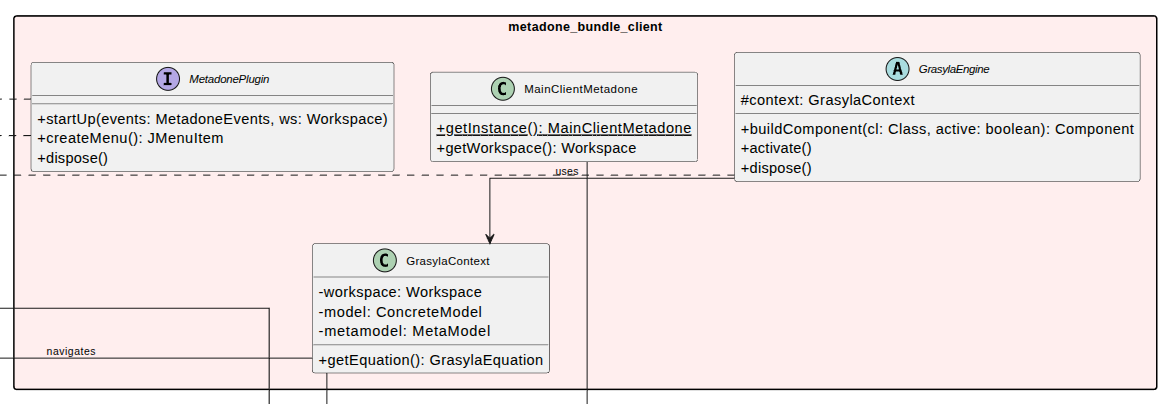
\includegraphics[width=0.9\textwidth]{img/architecture/bundle-client.png}
\caption{Bundle client}
\label{bundle-client}
\end{figure}

%\subsection{Intégration OSGi et point d'entrée}

%Conformément au modèle de composants OSGi, le bundle présente une classe \texttt{MetadoneActivator} qui instancie deux trackers : \texttt{ClientBusinessTracker} surveille l'apparition du service \texttt{Workspace} dans le registre OSGi, et \texttt{PluginTracker} détecte dynamiquement les plugins enregistrés par d'autres bundles.

\subsection{Système de plugins}

MetaDONE adopte une architecture orientée plugins pour garantir son extensibilité. Tout plugin implémente l'interface \texttt{MetadonePlugin}, qui impose quatre responsabilités : fournir un nom, contribuer un élément de menu Swing, réagir aux changements de workspace via \texttt{startUp} et libérer ses ressources via \texttt{dispose}.

La classe abstraite \texttt{AbstractMetadonePlugin} fournit une implémentation de base : elle souscrit automatiquement aux événements \texttt{WorkspaceChanged} afin de maintenir sa référence vers le workspace courant à jour. Chaque plugin est déployé dans son propre bundle OSGi et expose un \texttt{AbstractPluginActivator} qui l'enregistre dans le
registre de services au démarrage. Le \texttt{PluginTracker} du bundle client détecte ces enregistrements et intègre les menus correspondants dans l'interface principale sans nécessiter de recompilation ni de redémarrage de l'application.

\subsection{Abstraction de rendu}

Pour découpler la logique d'affichage des technologies d'interface graphique sous-jacentes, le bundle introduit une abstraction de rendu structurée en trois interfaces centrales.
\begin{itemize}
    \item L'interface \texttt{Context} encapsule l'environnement d'évaluation d'une vue : workspace courant, modèle concret, méta-modèle et table de variables.
    \item L'interface \texttt{Engine} représente un composant capable de produire un élément d'interface à partir d'un contexte donné. Sa méthode \texttt{buildComponent(Class<C>, boolean)} est générique : selon que l'on passe \texttt{JComponent.class} ou \texttt{Widget.class} (NetBeans Visual Library), le même engine produit un widget Swing ou un nœud de graphe interactif. 
    \item Enfin, l'interface \texttt{Component<C>} encapsule le résultat produit et maintient un lien vers l'engine l'ayant construit.
\end{itemize}
Les engines s'organisent en arbre parent-enfant : un engine composite gère le cycle de vie de ses enfants (activation, disposition) de façon transparente.

\subsection{Le langage GraSyLa}
\label{sec:grasyla}

Présenté brièvement en section~\ref{sec:dsl-dsml}, GraSyLa (\emph{Graphical Symbolic Language}) est un DSML intégré au bundle client, dont le rôle est de décrire de façon déclarative comment visualiser les objets d'un modèle. Plutôt que de coder en dur la représentation graphique de chaque type d'objet, un plugin ou un utilisateur avancé rédige des \emph{équations GraSyLa} qui associent des motifs sur le modèle à des structures visuelles.

Une équation GraSyLa a la forme générale \texttt{motif => expression}, où le membre gauche désigne un \texttt{MetaObject} du métamodèle (filtrant par typage les objets concrets concernés) et le membre droit décrit la structure graphique à produire : boîtes imbriquées, libellés, arbres, arêtes de graphe, images SVG, etc. Ce mécanisme permet à un même objet d'être affiché différemment selon le
contexte dans lequel il est visualisé.

La structure formelle d'un script GraSyLa est décrite par son méta-modèle, présenté à la figure~\ref{grasyla}~\cite{techreportgrasylaversion2}. Ce méta-modèle est lui-même exprimé à l'aide des concepts de MetaL$_2$, illustrant ainsi la réflexivité de MetaDONE : le framework décrit son propre langage de visualisation avec ses propres
outils de méta-modélisation.

\begin{figure}[tp]
\centering
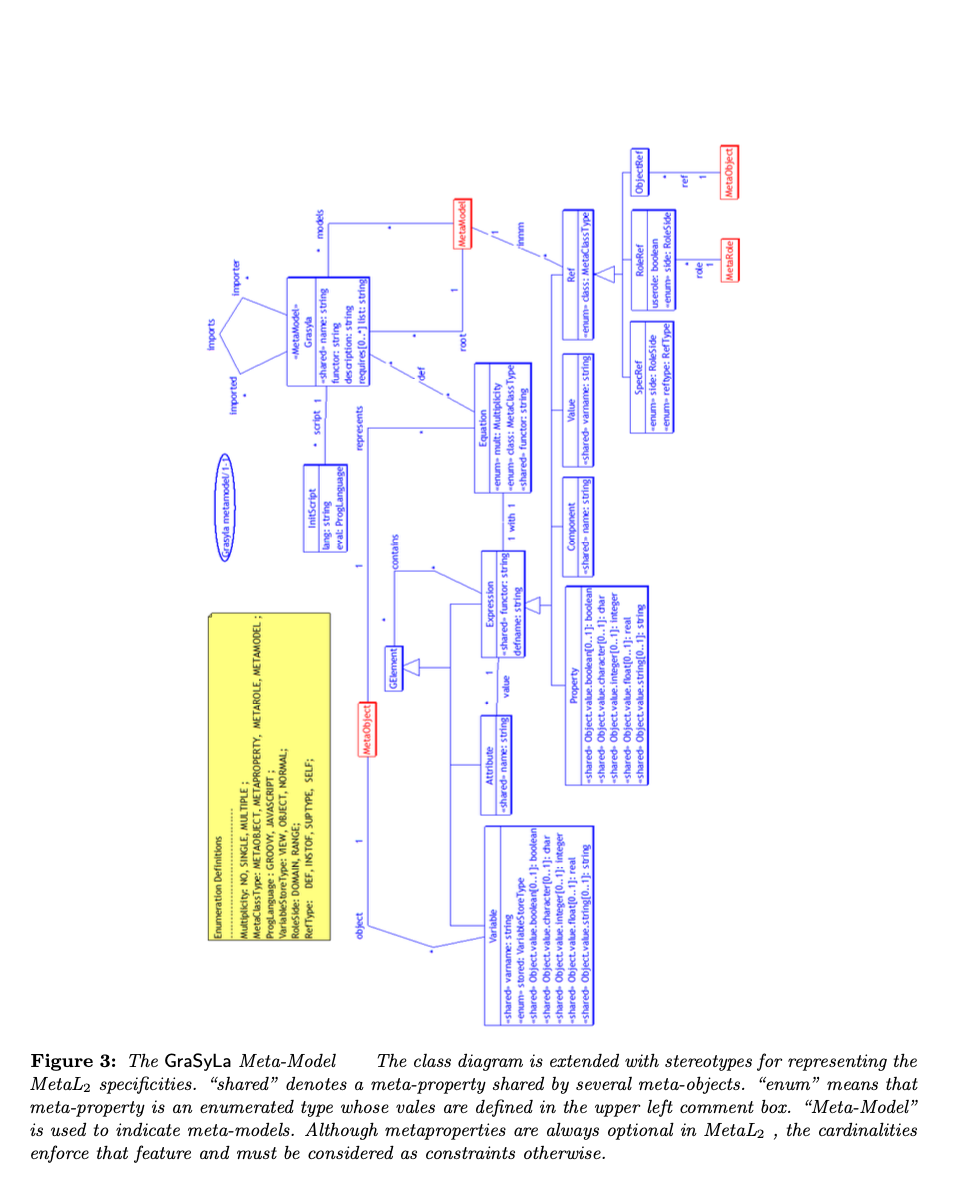
\includegraphics[width=\textwidth]{img/architecture/grasyla.png}
\caption{Méta-modèle de GraSyLa, exprimé en MetaL$_2$~\cite{techreportgrasylaversion2}}
\label{grasyla}
\end{figure}

Un script GraSyLa (\texttt{GrasylaMetamodel}) regroupe un ensemble d'équations (\texttt{Equation}) et un script d'initialisation optionnel (\texttt{InitScript}). Chaque équation possède un membre gauche
(\emph{LHS}) qui référence un \texttt{MetaObject} via la relation
\texttt{represents}, et un membre droit (\emph{RHS}) constitué d'un
arbre d'\texttt{Expression}. Cet arbre peut contenir des composants
(\texttt{Component}), des attributs visuels (\texttt{Attribute}), des
variables (\texttt{Variable}) et des propriétés (\texttt{Property}).
Les références au modèle sont typées : \texttt{ObjectRef} pointe vers
un objet concret, \texttt{RoleRef} vers un rôle, et \texttt{SpecRef}
vers une spécification.


L'interprétation d'un script GraSyLa repose sur deux composants principaux. Le \texttt{GrasylaContext} maintient l'état d'évaluation : workspace, modèle courant, méta-modèle, variables locales et équation sélectionnée. Le \texttt{GrasylaInterpreter}, qui étend \texttt{GrasylaEngine} et implémente \texttt{EngineInterpreter}, sélectionne la meilleure équation pour un objet donné puis délègue la construction du composant graphique aux engines spécialisés.

Ces engines spécialisés sont regroupés en plusieurs familles~:
\begin{itemize}
    \item \textbf{Engines Swing} (\texttt{JBoxEngine}, \texttt{JTreeEngine}, \texttt{JTableEngine}, \texttt{JComboBoxEngine}, etc.) : produisent des composants \texttt{JComponent} pour l'affichage dans des panneaux Swing classiques.
    \item \textbf{Engines Visual Library} (\texttt{GraphEngine}, \texttt{VLBoxEngine}, \texttt{VLEdgeEngine}, \texttt{VLShapeEngine}, etc.) : produisent des widgets NetBeans Visual Library pour l'affichage de graphes interactifs avec ancres, routeurs et formes personnalisées.
    \item \textbf{Engines logiques} : \texttt{IfEngine}, \texttt{GuardEngine}, \texttt{MatchEngine}, \texttt{OrEngine}, \texttt{NotEngine} permettent d'exprimer des conditions sur le modèle directement dans le script.
    \item \textbf{Engines de structure} : \texttt{ListEngine}, \texttt{GroupEngine}, \texttt{ReduceEngine}, \texttt{HeadEngine}, \texttt{TailEngine} permettent d'itérer sur des collections d'objets ou de rôles.
    \item \textbf{Engines de référence} (\texttt{CORefObjectEngine}, \texttt{MORefObjectEngine}, \texttt{MRRefRoleEngine}) : naviguent dans le modèle pour accéder aux objets concrets, aux méta-objets ou aux
    rôles référencés.
    \item \textbf{Engines de valeur} (\texttt{ValueEngine},
    \texttt{UpdaterEngine}, \texttt{MutableValue}) : lisent et modifient les propriétés d'un objet concret, propageant les changements via le système d'événements.
\end{itemize}

GraSyLa souscrit au système d'événements de MetaDONE : lorsqu'un objet est modifié ou supprimé, les engines actifs se rafraîchissent automatiquement sans intervention explicite du code applicatif.

\subsection{Dialogues Swing}

Le bundle fournit un ensemble de dialogues Swing couvrant les opérations courantes sur le méta-modèle et le modèle concret.

Les \emph{browsers} \texttt{BrowserMetal2} et \texttt{BrowserMetal1} présentent respectivement le méta-modèle (couche M2) et le modèle concret (couche M1) sous forme d'arbres navigables. Chaque nœud de l'arbre correspond à un concept précis : \texttt{NodeRoot\_MetaModel}, \texttt{NodeRoot\_MetaObject}, \texttt{NodeRoot\_MetaRole} pour M2 ; \texttt{NodeTypes}, \texttt{NodeProperties}, \texttt{NodeDomain}, \texttt{NodeInstances} pour M1.

Les éditeurs de méta-objets (\texttt{PanelMetaModel}, \texttt{PanelMetaObject}, \texttt{PanelMetaProperty}, \texttt{PanelMetaRole}) permettent de créer et modifier les éléments du méta-modèle. Pour les objets concrets, le \texttt{DialogConcreteObject} est construit dynamiquement par un \texttt{Builder} qui inspecte les méta-propriétés et méta-rôles de l'objet pour générer les widgets appropriés : un panel par type primitif (String, Integer, Float, Boolean, Char) en cardinalité 1 ou N, et des panels dédiés pour les rôles domain et range.

\subsection{Parsers et importeurs}

Le bundle intègre deux parsers. Le premier, composé de
\texttt{GrasylaLexer} et \texttt{GrasylaParser}, analyse les scripts GraSyLa et produit un AST (\emph{Abstract Syntax Tree}) dont les nœuds, \texttt{AST\_script}, \texttt{AST\_equation}, \texttt{AST\_expression},
\texttt{AST\_ref}, sont ensuite interprétés par le moteur GraSyLa. Le second, composé de \texttt{KM3Lexer} et \texttt{KM3Parser}, permet d'importer des méta-modèles au format KM3, un format textuel compatible avec les outils de la famille ATL/Kermeta.

Plusieurs importeurs, tous implémentant l'interface \texttt{Importer}, permettent d'alimenter le workspace à partir de sources externes : \texttt{GrasylaImporter} (scripts de visualisation), \texttt{MMDLImporter} (format natif MetaDONE), \texttt{KM3Importer} (méta-modèles KM3), \texttt{OWLImporter} (ontologies Web OWL) et \texttt{ModelImporter} (modèles génériques).

\section{Bundle \texttt{metadone\_bundle\_metabusiness}}

Le bundle \texttt{metadone\_bundle\_metabusiness} constitue la couche logique métier de MetaDONE (figure~\ref{bundle-MB}). Il implémente l'intégralité de MetaL$_2$ --- aussi bien la \textbf{couche méta-modèle} (niveaux M2 et M3 de MetaL~\cite{englebert_metal2}) que la \textbf{couche concrète} (niveau M1). Ces deux couches ne relèvent pas de deux langages distincts : elles correspondent à des niveaux d'instanciation au sein de MetaL$_2$, toutes deux construites sur le substrat de MetaL$_1$ fourni par \texttt{metadone\_bundle\_repository} (section~\ref{sec:repository}). Il fournit également l'ensemble des services sur lesquels s'appuient le bundle client et les
plugins : gestion du workspace, navigation dans les modèles, propagation des
événements et gestion de l'historique.

\begin{figure}[h]
\centering
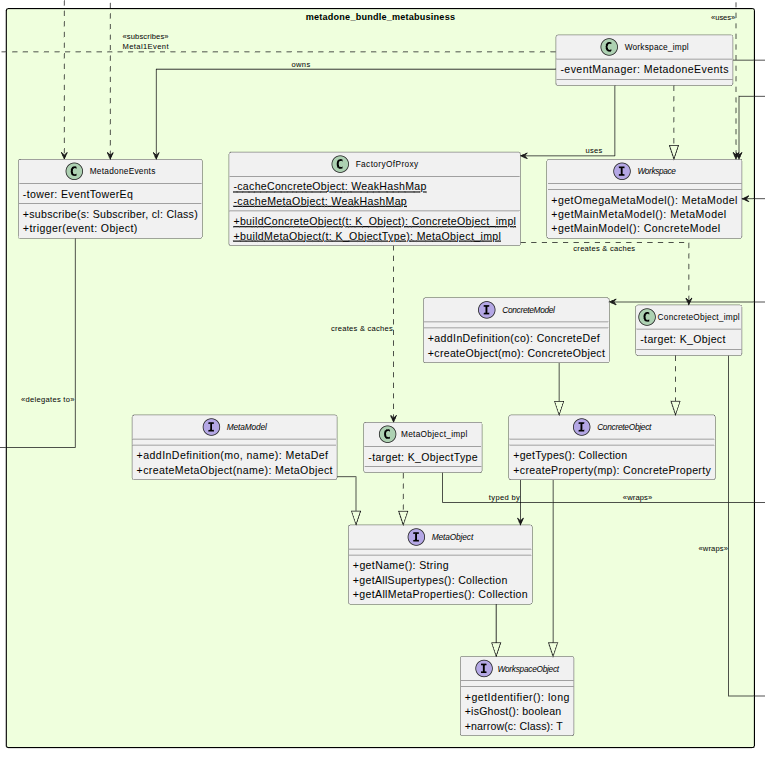
\includegraphics[width=0.7\textwidth]{img/architecture/bundle-MB.png}
\caption{Bundle metabusiness}
\label{bundle-MB}
\end{figure}

\subsection{Le patron Proxy : des interfaces sur des \texttt{DataObject}}
\label{sec:proxy}
Le premier principe architectural de ce bundle est l'usage systématique du patron de conception \textit{Proxy}. Chaque entité manipulée à travers les interfaces de MetaL$_2$ n'est pas un objet autonome : c'est un proxy léger qui encapsule un DataObject du bundle repository. Que l'entité soit un MetaObject, un MetaRole, un ConcreteObject ou un ConcreteRole, elle repose en dernière analyse sur un DataObject de MetaL$_1$, dont elle interprète les facettes à travers une interface
de plus haut niveau.

La classe abstraite \texttt{WorkspaceObject\_impl} constitue la base commune de
tous ces proxies. Elle maintient une référence vers le \texttt{Workspace\_impl}
courant et fournit l'opération de conversion sécurisée \texttt{narrow(Class<T>)},
qui tente de transtyper le proxy vers une interface plus spécifique et lève une
\texttt{BadPreCondition} si le transtypage est invalide.

La classe \texttt{FactoryOfProxy} centralise la création et la mise en cache des
proxies. Elle maintient des \texttt{WeakHashMap} associant chaque K\_Object ou
K\_ObjectType du repository à son proxy correspondant, garantissant que le même
DataObject produit toujours le même objet proxy. Ce cache à références faibles
permet au ramasse-miettes de récupérer les proxies inutilisés sans intervention
explicite.

\subsection{Implémentation de la couche méta-modèle (M2/M3)}
\label{sec:impl-metamodel}

La couche méta-modèle de MetaL$_2$ --- niveaux M2 et M3 de MetaL --- définit
les metaclasses qui permettent de décrire des domaines. Conformément à la
spécification formelle~\cite{englebert_metal2}, MetaObject, MetaRole, MetaProperty
et MetaModel héritent tous de MetaObject (sauf MetaObject lui-même), et MetaRole
est à la fois un type d'objet et un type de propriété.

La distinction clé avec la couche concrète réside dans la couche de MetaL$_1$
mobilisée : la couche méta-modèle s'appuie sur les \textbf{types} de MetaL$_1$
(K\_ObjectType, K\_PropertyType), là où la couche concrète s'appuie sur les
\textbf{instances} (K\_Object, K\_Property)~\cite{englebert_metal1}.

Dans l'implémentation, chaque concept correspond à une classe \texttt{*\_impl}
wrappant une facette de type du DataObject sous-jacent :

\begin{itemize}
  \item \texttt{MetaObject\_impl} encapsule un K\_ObjectType : un méta-objet est
    un type d'objet au sens du kernel, capable d'avoir des instances (K\_Object).
  \item \texttt{MetaRole\_impl} encapsule un K\_PropertyType : un méta-rôle est
    un type de propriété binaire orientée entre deux K\_ObjectType.
  \item \texttt{MetaProperty\_impl} encapsule également un K\_PropertyType
    spécialisé pour les attributs.
  \item \texttt{MetaDef\_impl} encapsule un K\_Property reliant un K\_ObjectType
    (l'objet membre, en position de domaine) à un K\_Object (le modèle, en position
    de range) ; il matérialise la relation \textit{PartWhole} de la spécification
    formelle~\cite{englebert_metal2}.
\end{itemize}

\texttt{MetaModel\_impl} étend \texttt{MetaObject\_impl} : un méta-modèle est
lui-même un méta-objet. Au niveau du kernel, il est représenté par un K\_ObjectType
avec la sémantique supplémentaire de conteneur de méta-objets.

\subsection{Le méta-méta-modèle Omega}

Un aspect fondamental de MetaL est que le niveau M3 est \textbf{réflexif} : les
metaclasses (MetaObject, MetaModel, MetaRole, MetaProperty) sont des instances
d'elles-mêmes~\cite{englebert_metal2}. Contrairement au MOF où M3 est
simplement \og conforme à lui-même \fg{}, MetaL en fait une \og vraie instance de
lui-même \fg{} --- une propriété formalisée dans~\cite{englebert_metal2}.

Le méta-modèle Omega, accessible via \texttt{Workspace.getOmegaMetaModel()},
matérialise ce niveau M3 dans MetaDONE. Il contient, en tant que MetaObject
ordinaires, les types primitifs du framework (String, Integer, Float, Boolean,
Char) ainsi que les metaclasses du framework elles-mêmes~: chacune est instance
d'elle-même --- \texttt{MetaObject} est instance de \texttt{MetaObject},
\texttt{MetaRole} est instance de \texttt{MetaRole}, \texttt{MetaProperty} est
instance de \texttt{MetaProperty}, et \texttt{MetaModel} est instance de
\texttt{MetaModel}.

Le méta-modèle principal de l'utilisateur, accessible via
\texttt{getMainMetaModel()}, est une instance de MetaModel (défini dans Omega) :
c'est le niveau M2. Les modèles concrets qui en sont instances constituent le
niveau M1.

\subsection{Implémentation de la couche concrète (M1)}
\label{sec:impl-concret}

Comme rappelé en section~\ref{sec:metal1}, MetaL$_1$ se limite au \texttt{DataObject}
et à ses facettes : aucun des concepts \texttt{ConcreteObject}, \texttt{ConcreteRole},
\texttt{ConcreteProperty} ou \texttt{ConcreteModel} n'appartient à cette couche. Tous
relèvent de MetaL$_2$~\cite{englebert_metal2}, au même titre que \texttt{MetaObject},
\texttt{MetaRole}, \texttt{MetaProperty} et \texttt{MetaModel}. La distinction interne à
MetaL$_2$ entre couche méta-modèle et couche concrète se traduit dans le choix des facettes
de MetaL$_1$ sur lesquelles elle s'appuie : la couche méta-modèle utilise les facettes de
\textbf{type} (\texttt{K\_ObjectType}, \texttt{K\_PropertyType}), la couche concrète celles
d'\textbf{instance} (\texttt{K\_Object}, \texttt{K\_Property})~\cite{englebert_metal1}.

Chaque concept de la couche concrète correspond à une classe \texttt{*\_impl} encapsulant
la facette appropriée :

\begin{itemize}
  \item \texttt{ConcreteObject\_impl} encapsule un K\_Object : un objet concret
    est une instance de K\_Object dont les types --- via la relation \textit{typeo}
    de MetaL$_1$ --- sont les K\_ObjectType correspondant aux MetaObject du
    méta-modèle.
  \item \texttt{ConcreteRole\_impl} encapsule un K\_Property et matérialise un
    lien concret entre deux ConcreteObject, instance d'un MetaRole.
  \item \texttt{ConcreteProperty\_impl} encapsule un K\_Property spécialisé
    portant une valeur primitive.
  \item \texttt{ConcreteDef\_impl} encapsule un K\_Property reliant un K\_Object
    (l'objet concret) à un K\_Object (le modèle), matérialisant la relation
    \textit{PartWhole} au niveau M1.
\end{itemize}

La réflexivité de MetaL$_2$ s'étend au niveau M1 : \texttt{ConcreteModel\_impl}
étend \texttt{ConcreteObject\_impl}, de sorte qu'un modèle concret est lui-même
un objet concret~\cite{englebert_metal2}. Il peut donc avoir des types,
des propriétés et participer à des rôles au même titre que n'importe quel élément
du modèle. C'est précisément cette uniformité qui permet à MetaDONE de stocker
ses scripts GraSyLa --- eux-mêmes des ConcreteObject --- dans le modèle et de les
manipuler avec les mêmes APIs que n'importe quel modèle utilisateur.

\section{Bundle \texttt{metadone\_bundle\_repository}}
\label{sec:repository}

Le bundle \texttt{metadone\_bundle\_repository} constitue la couche de persistance de MetaDONE (figure~\ref{bundle-repo}). Il définit un modèle de stockage minimaliste et générique --- le \emph{kernel} --- sur lequel reposent toutes les abstractions de MetaL$_1$ et MetaL$_2$ décrites précédemment. Ce bundle est purement abstrait : il ne contient que des interfaces et une classe abstraite, sans aucune dépendance vers une technologie de persistance concrète. Deux implémentations interchangeables en sont dérivées, présentées en fin de section.

\begin{figure}[h]
\centering
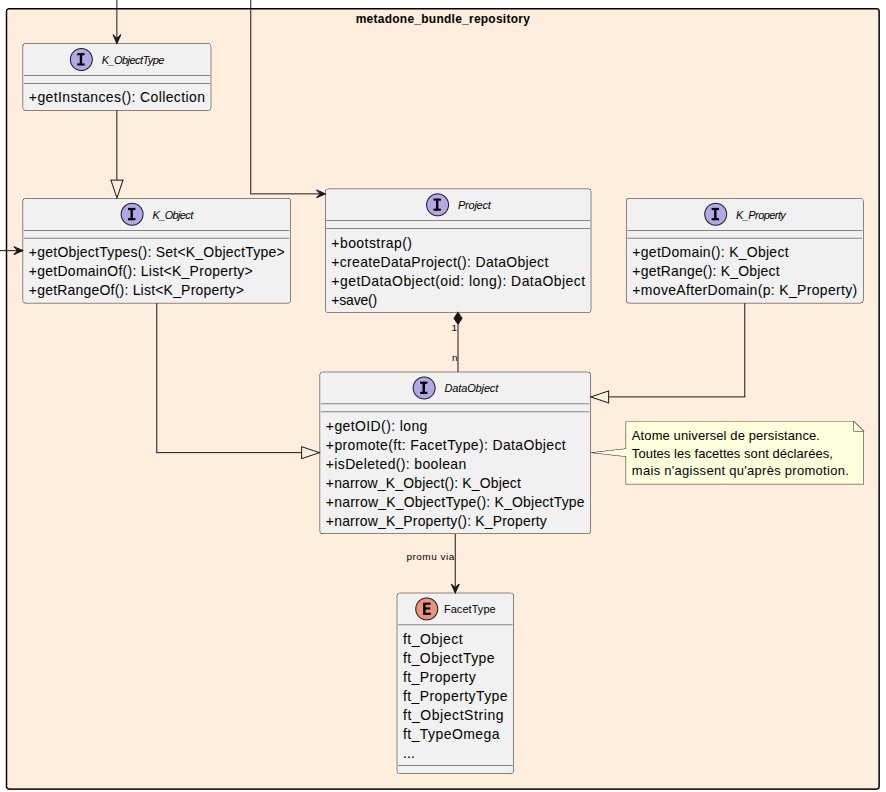
\includegraphics[width=0.7\textwidth]{img/architecture/bundle-repo.png}
\caption{Bundle repository}
\label{bundle-repo}
\end{figure}

\subsection{L'unité atomique : le \texttt{DataObject}}

Le \texttt{DataObject} est l'entité fondamentale du kernel. Chaque
élément du modèle, qu'il soit \texttt{MetaObject}, \texttt{MetaRole},
\texttt{ConcreteObject} ou \texttt{ConcreteProperty}, est en dernière analyse un \texttt{DataObject} persisté. Comme montré en
section~\ref{sec:impl-metamodel}, les classes \texttt{*\_impl} du bundle
métier sont toutes des proxies encapsulant un \texttt{DataObject}.

L'interface \texttt{DataObject} est remarquablement large : elle étend
simultanément l'ensemble des interfaces de facettes du kernel
(\texttt{K\_Common}, \texttt{K\_Object}, \texttt{K\_ObjectType},
\texttt{K\_Property}, \texttt{K\_PropertyType}, \texttt{K\_ObjectString},
\texttt{K\_ObjectInteger}, etc.), soit une quinzaine d'interfaces. Un
\texttt{DataObject} possède donc potentiellement toutes les capacités du
kernel, mais celles-ci ne sont activées qu'à la demande, via le mécanisme
de promotion.

\subsection{Le modèle de facettes et la promotion}

La flexibilité du kernel repose sur le concept de \emph{facette}. Plutôt
que de créer des types d'objets distincts pour chaque rôle possible, un
\texttt{DataObject} commence avec un ensemble vide de facettes actives et
se voit progressivement \emph{promu} vers de nouvelles capacités par
l'appel à \texttt{promote(FacetType)}. Cette promotion est irréversible
et cumulative : un objet peut acquérir plusieurs facettes compatibles.

L'enum \texttt{FacetType} liste les dix-sept facettes disponibles
(tableau~\ref{tab:facettypes}) et définit pour chacune sa
\emph{fermeture}, c'est-à-dire l'ensemble des facettes préalablement
requises. Par exemple, la promotion vers
\texttt{ft\_ObjectType} requiert \texttt{ft\_Common} et \texttt{ft\_Object},
et la promotion vers \texttt{ft\_PropertyTypePi} requiert \texttt{ft\_Common},
\texttt{ft\_Property} et \texttt{ft\_PropertyType}. Cette hiérarchie de
dépendances garantit la cohérence du modèle kernel.

\begin{table}[h]
\centering
\begin{tabular}{ll}
\hline
\textbf{Facette} & \textbf{Sémantique} \\
\hline
\texttt{ft\_Common} & Base commune à tout DataObject \\
\texttt{ft\_Object} & Objet pouvant avoir des types et des rôles \\
\texttt{ft\_ObjectType} & Type pouvant avoir des instances \\
\texttt{ft\_Property} & Lien orienté entre deux objets \\
\texttt{ft\_PropertyType} & Type de lien \\
\texttt{ft\_PropertyTypePi} & Type de lien racine (singleton) \\
\texttt{ft\_ObjectString/Integer/Float/Boolean/Char} & Valeur primitive \\
\texttt{ft\_TypeString/Integer/Float/Boolean/Char/Omega} & Type primitif prédéfini \\
\hline
\end{tabular}
\caption{Principales facettes du kernel MetaDONE}
\label{tab:facettypes}
\end{table}

\subsection{La hiérarchie des interfaces \texttt{K\_*}}

Chaque facette correspond à une interface \texttt{K\_*} qui expose les
opérations associées :

\begin{itemize}
    \item \texttt{K\_Object} : accès aux types de l'objet
    (\texttt{getObjectTypes()}), aux propriétés dont il est domaine
    (\texttt{getDomainOf()}) ou codomaine (\texttt{getRangeOf()}).
    \item \texttt{K\_ObjectType} : accès aux instances du type
    (\texttt{getInstances()}) et navigation dans la hiérarchie de
    sous-types.
    \item \texttt{K\_Property} : accès au domaine (\texttt{getDomain()})
    et au codomaine (\texttt{getRange()}) du lien, gestion de l'ordre
    dans les listes (\texttt{moveAfterDomain()},
    \texttt{moveLastRange()}).
    \item \texttt{K\_PropertyType} : type d'un lien, associant un type
    de domaine et un type de codomaine.
    \item \texttt{K\_ObjectString}, \texttt{K\_ObjectInteger}, etc. :
    stockage d'une valeur primitive du type correspondant.
\end{itemize}

Le transtypage vers une interface précise s'effectue via les méthodes
\texttt{narrow\_K\_*()} du \texttt{DataObject}, qui retournent
\texttt{null} si la facette requise n'est pas active. L'invocation
ultérieure d'une opération sur une facette inactive (par exemple
\texttt{getDomain()} sur un DataObject sans facette \texttt{Property})
lève alors une \texttt{BadFacet}.

\subsection{Les relations de typage et de sous-typage}

Deux relations N-N fondamentales structurent le kernel.
\texttt{NN\_typeof} matérialise le lien \emph{instance-de} entre un
\texttt{K\_Object} et un \texttt{K\_ObjectType} : c'est par cette
relation qu'un \texttt{ConcreteObject} est lié à son
\texttt{MetaObject}. \texttt{NN\_subtype} matérialise le lien
\emph{sous-type-de} entre deux \texttt{K\_ObjectType} : c'est par cette
relation que l'héritage entre \texttt{MetaObject} est persisté.

Ces relations sont des objets explicites, ce qui permet de les naviguer dans les deux sens et de les
gérer via le cycle de vie standard (\texttt{PersistenceLifeCycle}).

\subsection{Le \texttt{Project} et le bootstrap}

Le \texttt{Project} est le conteneur racine de tous les
\texttt{DataObject}. Il joue deux rôles : celui de factory
(\texttt{FactoryData}) pour la création des entités, et celui de registre
des types primitifs prédéfinis. L'opération \texttt{bootstrap()} est
appelée à l'initialisation du projet et crée les singletons de types
primitifs (\texttt{K\_TypeInteger}, \texttt{K\_TypeString},
\texttt{K\_TypeFloat}, \texttt{K\_TypeBoolean}, \texttt{K\_TypeChar} et
\texttt{K\_TypeOmega}) ainsi que le type racine de toutes les propriétés \texttt{K\_PropertyTypePi}.

La classe abstraite \texttt{AbstractProject} fournit l'infrastructure
événementielle du kernel. Elle maintient un \texttt{EventTower<Metal1Event>}
et déclenche des événements de bas niveau à chaque modification
structurelle : \texttt{EventCreateDataObject} à la création,
\texttt{EventLink} au lien de sous-typage ou de typage,
\texttt{EventWillDelete} avant suppression, \texttt{EventChange} et
\texttt{EventChangeFacet} lors de modifications. Ces événements sont
capturés par \texttt{Workspace\_impl} pour être traduits en événements
MetaL$_2$ plus riches.

\subsection{Implémentation JPA2 :
\texttt{metadone\_bundle\_repository\_jpa2}}

Le bundle \texttt{metadone\_bundle\_repository\_jpa2} fournit une
implémentation relationnelle du kernel, reposant sur
\emph{Apache OpenJPA 2.3.0}. La classe \texttt{DataObjectJPA2} est
annotée \texttt{@Entity} et mappée vers une table relationnelle unique par
un schéma de type \emph{single-table inheritance}.

La sérialisation de l'ensemble de facettes actives d'un
\texttt{DataObject} est réalisée via la classe \texttt{Facets}, qui
encode un \texttt{EnumSet<FacetType>} en un entier par manipulation de
bits (\texttt{jpaExtern}) et le reconstitue à la lecture
(\texttt{jpaBuild}). Ce choix de représentation compacte réduit
l'empreinte mémoire et le coût d'accès en base.

Les relations N-N (\texttt{NN\_typeofJPA2}, \texttt{NN\_subtypeJPA2})
sont mappées avec des annotations \texttt{@OneToMany} et
\texttt{@ManyToOne}. Les requêtes nécessitant un filtrage sur les types
ou les sous-types utilisent l'API JPA Criteria, évitant la construction
de JPQL sous forme de chaînes de caractères. La classe
\texttt{ProjectJPA2} gère la transaction via un \texttt{EntityManager}
JPA standard, encapsulé dans \texttt{TransactionJPA2}.

\subsection{Implémentation ObjectDB :
\texttt{metadone\_bundle\_repository\_odb}}

Le bundle \texttt{metadone\_bundle\_repository\_odb} fournit une
implémentation alternative reposant sur \emph{ObjectDB 2.5.7}, une base
de données orientée objet pour Java, compatible JPA. La classe
\texttt{DataObjectODB} utilise les mêmes annotations JPA que son
homologue JPA2 (\texttt{@Entity}, \texttt{@Id}, \texttt{@OneToMany},
etc.), ObjectDB implémentant nativement la spécification JPA sans couche
ORM intermédiaire.

L'intérêt de cette implémentation réside dans l'alignement naturel entre
le modèle objet Java et le moteur de stockage : les objets sont persistés
tels quels, sans transformation relationnelle. Cela simplifie les
stratégies de mapping et peut réduire l'impedance objet-relationnel
présente dans l'implémentation JPA2. La transaction est gérée par
\texttt{TransactionODB}, qui encapsule le mécanisme de transaction propre
à ObjectDB.

\subsection{Substitution par OSGi}

Les deux implémentations exposent un service \texttt{FactoryProject} dans
le registre OSGi via leur \texttt{Activator} respectif. Le bundle
\texttt{metadone\_bundle\_metabusiness} découvre ce service à travers son
\texttt{RepositoryTracker} : selon le bundle repository démarré par
Equinox, l'implémentation JPA2 ou ODB est sélectionnée de manière transparente,
sans que le reste de l'application n'en soit informé. Ce mécanisme
illustre concrètement le bénéfice de l'architecture OSGi pour
l'interchangeabilité des composants à l'exécution.

\section{Bundle \texttt{metadone\_common}}

Le bundle \texttt{metadone\_common} est une bibliothèque d'infrastructure
partagée par l'ensemble des bundles de MetaDONE (figure~\ref{bundle-common}). Il ne contient aucune
logique métier, mais fournit les abstractions transversales sur lesquelles
repose toute l'architecture : système de notification, utilitaires de
collections et hiérarchie d'exceptions.

\begin{figure}[h]
\centering
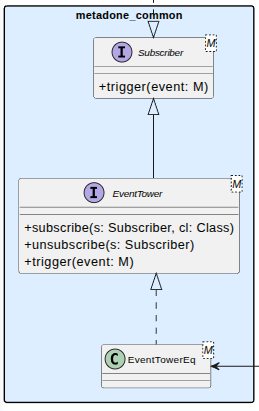
\includegraphics[width=0.3\textwidth]{img/architecture/bundle-common.png}
\caption{Bundle common}
\label{bundle-common}
\end{figure}

\subsection{Le système publish-subscribe}

Le sous-package \texttt{publish\_subscribe} définit le mécanisme de
notification réactif utilisé à travers tous les niveaux de
l'architecture : \texttt{AbstractProject} l'utilise pour les événements
kernel (\texttt{Metal1Event}), \texttt{MetadoneEvents} l'utilise pour les
événements métier (\texttt{Metal2Event}), et les engines GraSyLa
s'abonnent aux changements du workspace pour se rafraîchir
automatiquement.

Le contrat central est l'interface \texttt{EventTower<M>}, qui étend
elle-même \texttt{Subscriber<M>} : une tour d'événements est donc aussi
un souscripteur, ce qui permet de composer et chaîner des tours.
L'abonnement est filtré à deux niveaux : par \emph{type Java} de
l'événement (via \texttt{Class<T>}) et, optionnellement, par
\emph{prédicat} (\texttt{MapFct<T, Boolean>}).

Trois implémentations de \texttt{EventTower} sont proposées :
\begin{itemize}
    \item \texttt{EventTowerNormal} : implémentation de base maintenant
    une liste de nœuds d'abonnement indexés par classe d'événement.
    \item \texttt{EventTowerEq} : extension optimisée de
    \texttt{EventTowerNormal} qui reconnaît le motif de prédicat
    le plus fréquent dans MetaDONE --- tester l'égalité d'un attribut
    de l'événement à une valeur fixe (\texttt{MapFcts.Equal}) --- et
    les indexe dans une \texttt{HashMap} pour un dispatch en O(1) plutôt
    qu'une évaluation linéaire des prédicats. C'est cette implémentation
    qu'utilise \texttt{MetadoneEvents}.
    \item \texttt{EventTowerBuffer} : implémentation qui accumule les
    événements dans un tampon avant de les dispatcher, utile pour
    grouper des modifications en rafale.
\end{itemize}

La classe \texttt{AbstractSubscription} encapsule le cycle de vie d'un
abonnement (souscription et désabonnement) et sert de base à
\texttt{Subscription} (abonnement simple) et
\texttt{SubscriberHandler} (abonnement avec délégation à un
\texttt{Consumer} fonctionnel).

\subsection{Utilitaires}

Le sous-package \texttt{util} regroupe des structures de données et des
fonctions utilitaires employées intensivement dans les couches
supérieures.

Parmi les structures notables dans le contexte de l'optimisation,
\texttt{CacheCallFunction<Arg, Ret>} est une structure de mémoïsation
générique : elle associe une valeur de retour à chaque argument
d'appel dans une \texttt{HashMap} et peut être désactivée par
configuration pour désactiver le cache sans modifier le code appelant.
\texttt{LazySet<E>} est un proxy copy-on-write sur un \texttt{Set} : il
référence le set original sans le copier tant qu'aucune modification
n'est effectuée, ce qui réduit l'allocation mémoire dans les scénarios
de lecture dominante.

Les autres utilitaires couvrent les besoins courants : \texttt{Pair<A,B>}
et \texttt{BiDir<A,B>} pour les associations bidirectionnelles,
\texttt{MapFct<A,B>} comme interface fonctionnelle précédant les lambdas
Java 8, \texttt{ImmutableList}, \texttt{ListUtil}, \texttt{SetUtil} et
\texttt{IteratorUtil} pour la manipulation de collections, et
\texttt{Chrono} pour la mesure des temps d'exécution.

\subsection{Exceptions}

La hiérarchie d'exceptions maison couvre les cas les plus fréquents :
\texttt{BadPreCondition} (et sa spécialisation \texttt{NullArgument})
pour les violations de contrats d'entrée, \texttt{InternalException}
pour les erreurs internes inattendues, \texttt{FailedOperation} pour les
opérations échouées de façon récupérable, et \texttt{NotYetImplemented}
comme marqueur de code à compléter.

\section[Synthèse]{Synthèse : réflexivité et omniprésence des \texttt{DataObject}}
\label{sec:reflexivite}

Les quatre bundles présentés dans ce chapitre forment un système cohérent
dont deux propriétés architecturales transversales méritent d'être mises
en lumière avant d'aborder l'optimisation : la \emph{réflexivité} du
modèle à niveaux, et l'\emph{omniprésence} du \texttt{DataObject} comme substrat universel de persistance.

\subsection{Une architecture réflexive}

La réflexivité de MetaDONE signifie que le framework se décrit lui-même
avec ses propres outils. Cette propriété se manifeste à plusieurs niveaux.

Au niveau de MetaL$_2$, \texttt{MetaModel} étend \texttt{MetaObject} : un
méta-modèle est lui-même un méta-objet, susceptible d'avoir des types,
des propriétés et des rôles. Le méta-modèle Omega, accessible via
\texttt{Workspace.getOmegaMetaModel()}, contient en tant que
\texttt{MetaObject} ordinaires les concepts de MetaL$_2$ lui-même ainsi que les types primitifs. MetaDONE utilise
donc ses propres APIs pour naviguer dans sa propre structure.

Au niveau de MetaL$_1$, \texttt{ConcreteModel} étend \texttt{ConcreteObject}
: un modèle concret est lui-même un objet concret, instance d'un
\texttt{MetaModel}. La hiérarchie est ainsi uniforme et récursive à
chaque niveau.

La conséquence la plus frappante de cette réflexivité est que les scripts
GraSyLa (le langage de description de vues présenté en
section~\ref{sec:grasyla}) sont eux-mêmes stockés dans le modèle MetaDONE sous forme de \texttt{ConcreteObject}. Une équation GraSyLa est une instance d'un \texttt{MetaObject} défini dans le méta-modèle Omega ;
ses membres gauche et droit sont accessibles et modifiables via les APIs
standard de MetaL$_1$. Le moteur de rendu, le langage de vue et les données
métier partagent ainsi le même substrat de représentation, sans
distinction de nature.

Cette uniformité est un atout de conception : elle permet de manipuler
n'importe quel aspect du système --- modèle, méta-modèle, scripts de
visualisation, configuration --- avec un seul ensemble d'APIs. Elle a
néanmoins une contrepartie directe sur les performances, que nous allons
à présent examiner.

\subsection{L'omniprésence du \texttt{DataObject}}

Le patron Proxy présenté en section~\ref{sec:impl-metamodel} a une
implication quantitative forte : en pratique, la quasi-totalité des
entités manipulées par MetaDONE sont des \texttt{DataObject} du kernel,
enveloppés dans des proxies sémantiques.

\begin{itemize}
    \item Chaque \texttt{MetaObject} est un proxy sur un
    \texttt{K\_ObjectType}, lui-même un \texttt{DataObject} promu
    \texttt{ft\_ObjectType}.
    \item Chaque \texttt{MetaRole} et \texttt{MetaProperty} sont des
    proxies sur un \texttt{K\_PropertyType}, soit un \texttt{DataObject}
    promu \texttt{ft\_PropertyType}.
    \item Chaque \texttt{ConcreteObject} est un proxy sur un
    \texttt{K\_Object}, soit un \texttt{DataObject} promu
    \texttt{ft\_Object}.
    \item Chaque \texttt{ConcreteRole} et \texttt{ConcreteProperty} sont
    des proxies sur un \texttt{K\_Property}, soit un \texttt{DataObject}
    promu \texttt{ft\_Property}.
    \item Chaque \texttt{MetaDef} et \texttt{ConcreteDef} sont des
    proxies sur un \texttt{K\_Property} reliant deux \texttt{DataObject}.
    \item Chaque nœud de l'arbre d'expression d'une équation GraSyLa est
    un \texttt{ConcreteObject}, donc lui aussi un \texttt{DataObject}.
\end{itemize}

Les seules entités qui ne sont pas directement des \texttt{DataObject}
sont les liaisons de typage (\texttt{NN\_typeof}) et de sous-typage
(\texttt{NN\_subtype}), qui sont des enregistrements de relation distincts mais qui sont eux-mêmes persistés et gérés par le kernel.

Il résulte de cette conception que l'ensemble du contenu d'un projet MetaDONE est représenté par un graphe homogène de \texttt{DataObject} liés entre
eux par des \texttt{K\_Property} (relations) et des
\texttt{NN\_typeof}/\texttt{NN\_subtype} (typage et héritage).

\subsection{Des algorithmes complexes sur un substrat homogène}

L'homogénéité du substrat, si elle simplifie la conception, engendre une
classe de problèmes de performance caractéristiques. Puisque toute
sémantique est encodée dans le graphe de \texttt{DataObject}, les
opérations logiquement simples requièrent des traversées récursives de ce
graphe.

L'opération \texttt{getMOByName}, par exemple, doit naviguer
récursivement dans l'arbre des \texttt{MetaModel} en traversant les
\texttt{K\_Property} de définition, puis filtrer les \texttt{MetaObject}
par nom --- une recherche linéaire sur des \texttt{DataObject}. Dans les
modèles de taille réelle, cette opération est appelée de manière répétée
lors du bootstrap, de l'import et du rendu GraSyLa.

L'opération \texttt{\_isInDefinition}, appelée à chaque ajout d'un
\texttt{ConcreteObject} dans un \texttt{ConcreteModel}, doit parcourir
l'ensemble des propriétés du modèle pour vérifier qu'un objet n'y est
pas déjà présent. Sans précaution, chaque appel à
\texttt{addInDefinition} déclenche un scan linéaire de l'ensemble de la
définition du modèle.

De même, les algorithmes de navigation des hiérarchies de types ---
\texttt{getAllSupertypes()}, \texttt{getAllSubtypes()},
\texttt{getAllMetaProperties()} --- doivent traverser les chaînes
\texttt{NN\_subtype} de manière récursive, ce qui dans une hiérarchie
profonde engendre un nombre d'accès aux \texttt{DataObject} croissant
avec la profondeur de l'arbre.

\subsection{Les optimisations comme réponse structurelle}

Les travaux d'optimisation conduits dans le cadre de ce mémoire
s'inscrivent directement dans ce contexte. Les principales interventions
portent sur la mise en cache stratégique des résultats de ces traversées
coûteuses.

Dans \texttt{ConcreteModel\_impl}, un cache de type
\texttt{WeakHashMap<ConcreteObject\_impl, Boolean>} mémorise les
résultats de \texttt{\_isInDefinition} : la vérification d'appartenance
passe ainsi d'un scan linéaire à un accès en O(1) pour les appels
ultérieurs. Ce cache est mis à jour de façon incrémentale lors de
\texttt{addInDefinition} --- sans nécessiter de re-scan --- et invalidé
lors de \texttt{removeFromDefinition}.

Dans \texttt{MetaModel\_impl}, la \texttt{CacheCallFunction} du bundle
\texttt{metadone\_common} est utilisée pour mémoïser les résultats de
\texttt{getMetaObjectsInDefinition}, indexés par l'OID du
\texttt{DataObject} sous-jacent. Cette clé d'indexation par OID est
précisément rendue possible par l'omniprésence des \texttt{DataObject} :
chaque entité possède un identifiant stable et unique dans le kernel,
directement accessible depuis le proxy.

L'usage de \texttt{WeakHashMap} dans les deux cas garantit que les
entrées de cache sont récupérées par le ramasse-miettes dès que le proxy
correspondant n'est plus référencé, évitant toute fuite mémoire dans un
système où les objets peuvent être supprimés à l'exécution.

Ces optimisations illustrent une tension fondamentale inhérente à l'architecture réflexive de MetaDONE : la généricité et l'uniformité du substrat \texttt{DataObject} sont des atouts de conception, mais transfèrent la complexité vers les algorithmes qui doivent interpréter et naviguer ce graphe homogène. Le chapitre suivant présente une analyse systématique de ces goulots d'étranglement et les stratégies mises en œuvre pour les résoudre.